\paragraph{概念}

\begin{itemize}
    \item 割点: 一个无向联通图中, 如果删去点u,该图联通数改变(不再是1),则该点为割点
    \item 点双连通图: 对于一个无向图, 其不拥有割点则为点双连通图
    \item 点双连通分量: 一个无向图的\textbf{极大}点双联通子图被称为点双联通分量
\end{itemize}

\paragraph{性质}

\begin{itemize}
    \item 点双(除两点一线的特殊情况)任意两点间都存在至少两条\textbf{点不重复}路径
    \item 点双(除两点一线的特殊情况)一定是边双,反之不一定
    \item 任意一个不是孤立点的割点都在至少两个点双中
    \item 任意一个不是割点的点,存在且只存在于一个点双中
\end{itemize}

\paragraph{样例四图片}

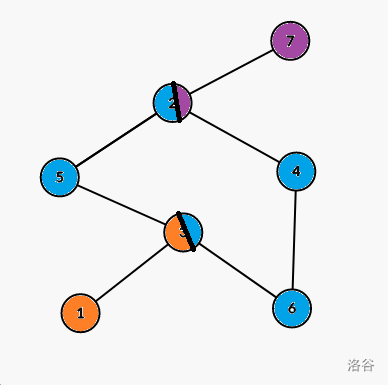
\includegraphics[width=0.4\textwidth]{img/luogu-P8435-1.png}
